\documentclass[final,dvipsnames]{beamer}

% ====================
% Packages
% ====================

\usepackage[T1]{fontenc}
\usepackage{tgbonum}
\usepackage[size=a0,orientation=portrait]{beamerposter}
\usetheme{gemini}
\usecolortheme{mit}
\usepackage{graphicx}
\usepackage{booktabs}
\usepackage{tikz}
\usetikzlibrary{trees, matrix, positioning, patterns, shapes, shadows, shapes.arrows, arrows.meta, shapes.multipart, decorations.pathreplacing, calc, tikzmark, shapes.geometric}
\usepackage{pgfplots}
\pgfplotsset{compat=1.14}
\pgfplotsset{every axis/.append style={very thick}}
\usepackage{pgf-pie}
\usepackage[binary-units]{siunitx}
\usepackage{anyfontsize}
\usepackage{amsmath}
\usepackage{mathdots}
\usepackage{mathtools}
\usepackage{bm}
\usepackage[normalem]{ulem}


% ====================
% Lengths
% ====================

% If you have N columns, choose \sepwidth and \colwidth such that
% (N+1)*\sepwidth + N*\colwidth = \paperwidth
\newlength{\sepwidth}
\newlength{\colwidth}
\setlength{\sepwidth}{0.025\paperwidth}
\setlength{\colwidth}{0.3\paperwidth}

\newcommand{\separatorcolumn}{\begin{column}{\sepwidth}\end{column}}

% ====================
% Title
% ====================

\title{\sout{Safe}Tix, The Best-Worst QR-Code Scanner}

\author{ \inst{1} \and Alexander Mattingley-Scott \inst{1}}

\institute[shortinst]{\inst{1} Heidelberg University}

% ====================
% Footer (optional)
% ====================

\footercontent{
	Binary Hacking 2024/25 \hfill
	\href{mailto:your.email@stud.uni-heidelberg.de}{tt249@stud.uni-heidelberg.de}}
% (can be left out to remove footer)

% ====================
% Logo (optional)
% ====================

% use this to include logos on the left and/or right side of the header:
%\logoright{\includegraphics[height=6cm]{}}
%\logoleft{\includegraphics[height=6cm]{}}

% ====================
% Body
% ====================

\begin{document}

\begin{frame}[t, fragile]
\begin{columns}[t]
\separatorcolumn

\begin{column}{\colwidth}

	\begin{block}{Motivation and Challenges}

		\begin{itemize}
			\item For our project, we decided to recreate a QR code scanner that mimics the behavior of SafeTix. 
			SafeTix, a digital ticketing system used by TicketMaster, claims to enhance security through dynamically rotating QR codes. 
			However, we found an article that takes a closer look at its implementation and reveals significant vulnerabilities that undermine its effectiveness.

			The Safetix system generates time-based one-time passwords (TOTPs) using an event-specific key and a customer-specific key, with a 15-second time step. 
			While this is meant to prevent duplication, the raw token containing this data is easily extractable from the web application’s source code. 
			In fact, TicketMaster logs the token directly to the browser console, making it trivial for attackers to capture and reuse it.
			This flaw enables unauthorized duplication, resale, or offline storage of tickets—effectively bypassing TicketMaster’s restrictions. 
			Additionally, there is uncertainty about the lifetime of raw tokens, raising concerns about the extent to which SafeTix can prevent ticket fraud.
			
			By recreating SafeTix, we aimed to make it a notch safer (not logging the ticket to the console) but keep a vulnerability that can be reverse engineered. 
			\item 
		\end{itemize}

	\end{block}


\end{column}

\separatorcolumn

\begin{column}{\colwidth}

	\begin{alertblock}{Methodology and Concept}

		How did you solve the problem.

		\begin{enumerate}
				\item First do this.
				\item Then this.
				\item Then that.
		\end{enumerate}

		\begin{figure}[h] % "h" means place here
			\centering
			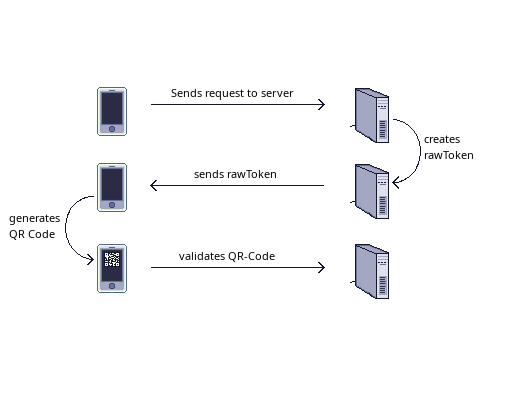
\includegraphics[width=0.9\textwidth]{Image_1.png} % Adjust width as needed
			\caption{The Program for dummies I guess ?.}
			\label{fig:sample}
		\end{figure}

		This solves the problem nicely! Citation\cite{goli_resprop_2020}

	\end{alertblock}

	\begin{block}{Details about X}

		Give some details about a specific part of your project you think is
		important or interesting.

	\end{block}

	\begin{block}{Details about Y}

		Same for another part.

	\end{block}

\end{column}

\separatorcolumn

\begin{column}{\colwidth}

	\begin{block}{Results}

		Show some of your results. For reversing tasks: show what you found about
		the target. For exploitation tasks: show to what results your topic can be
		used.

	\end{block}

	\begin{exampleblock}{Future Work}
		How would you improve on your work in the future?
		\begin{itemize}
			\item Make everything cleaner.
			\item Make everything faster.
			\item Make everything cheaper.
		\end{itemize}
	\end{exampleblock}

	\begin{block}{References}
		%\nocite{*}
		\footnotesize{\bibliographystyle{ieeetr}\bibliography{poster.bib}}
	\end{block}

\end{column}

\separatorcolumn
\end{columns}
\end{frame}

\end{document}
